% =====================================================================
%  Partie 4 -- Climat
% =====================================================================
\part{Climat}
Cette partie à pour but de présenter les mécanisme à l'oeuvre dans le rechauffement climatique via l'effet de serre. Pour cela, quelques précisions et une contextualisation des enjeux environementaux est effectué dans un premier temps.

\chapter{Contexte et enjeux environnementaux}
\section{Enjeux environnementaux}
\label{sec:enjeux}
 
Lorsqu'on parle d'enjeux environnementaux, on pense spontanément au
climat. C'est pourtant l'un des trois domaines à considérer,
étroitement liés les uns aux autres :
 
\begin{itemize}
    \item \textbf{le climat} : la succession des conditions météorologiques de la planète(température, humidité et pression de l'atmosphère) sur de longues périodes temporelle (à ne pas confondre avec la météo qui est sur le temps cours : quel temps ferat'il demain ?)
    \item \textbf{les ressources} : les stocks d'eau ou de
    ressources minérales et fossiles dont l'extraction a un coût environnemental
    \item \textbf{la santé} : A la fois humaine
    (pollution de l'air, îlots de chaleur, etc) et celle des écosystèmes (biodiversité,
    sols, milieux aquatiques)
\end{itemize}
 
Le secteur du bâtiment intervient sur ces trois plans : il émet des gaz à
effet de serre, de la construction comme à l'usage, il consomme de grandes quantités de matières premières en impactant ses écosystèmes, et il conditionne le confort et la santé des usagers
 
% ------------------------------------------------------------------
\section{Réchauffement climatique}
\label{sec:rechauffement}
 
La température moyenne à la surface du globe a augmenté d'environ 1.1\,°C par rapport à la période préindustrielle
(1850-1900), et cette hausse s'est nettement accélérée depuis le milieu
du \textsc{xx}\textsuperscript{e}~siècle, voir figure~\ref{fig:climat}. Le GIEC considère comme sans équivoque que l'influence humaine a réchauffé l'atmosphère, les océans et les terres\footfullcite{ipcc_climate_2021}.
 
\begin{figure}[htbp]
    \centering
    \includesvg[width=\linewidth]{figures/Climat.svg}
    \caption{Évolution de la température moyenne mondiale\cite{ipcc_climate_2021}.}
    \label{fig:climat}
\end{figure}
 
Le mécanisme physique à l'origine de ce réchauffement, l'effet de serre est détaillé par la suite.
 
 
% ------------------------------------------------------------------
\section{Ressources}
\label{sec:ressources}
 
Une croissance infinie de la consommation de matières est incompatible avec un monde aux ressources finies. Cette contrainte concerne directement la construction, grande consommatrice de granulats, de sable, de métaux et d'énergie fossile \footfullcite{jancovici-blain2021}, \footfullcite{bihouix-perriot2024}
 
% ------------------------------------------------------------------
\section{L'ère de l'Anthropocène}
\label{sec:anthropocene}
 
Le terme \emph{Anthropocène} désigne une période au cours de laquelle les activités humaines sont devenues une force capable de modifier le fonctionnement du système terrestre dans son ensemble.
 
Les travaux de Steffen\footfullcite{steffen_trajectory_2015} illustrent ce basculement en suivant, de 1750 à 2010, deux séries d'indicateurs. Les premiers décrivent le développement socio-économique
mondial : population, PIB, consommation d'énergie primaire, d'eau, d'engrais, urbanisation, transports, etc, voir figure~\ref{fig:anthropocene1}. Les seconds décrivent l'état du système terrestre : concentrations en gaz à effet de serre, acidification des océans, température de surface, perte de forêts tropicales, dégradation de la biosphère, etc, figure~\ref{fig:anthropocene2}.
 
\begin{figure}[htbp]
    \centering
    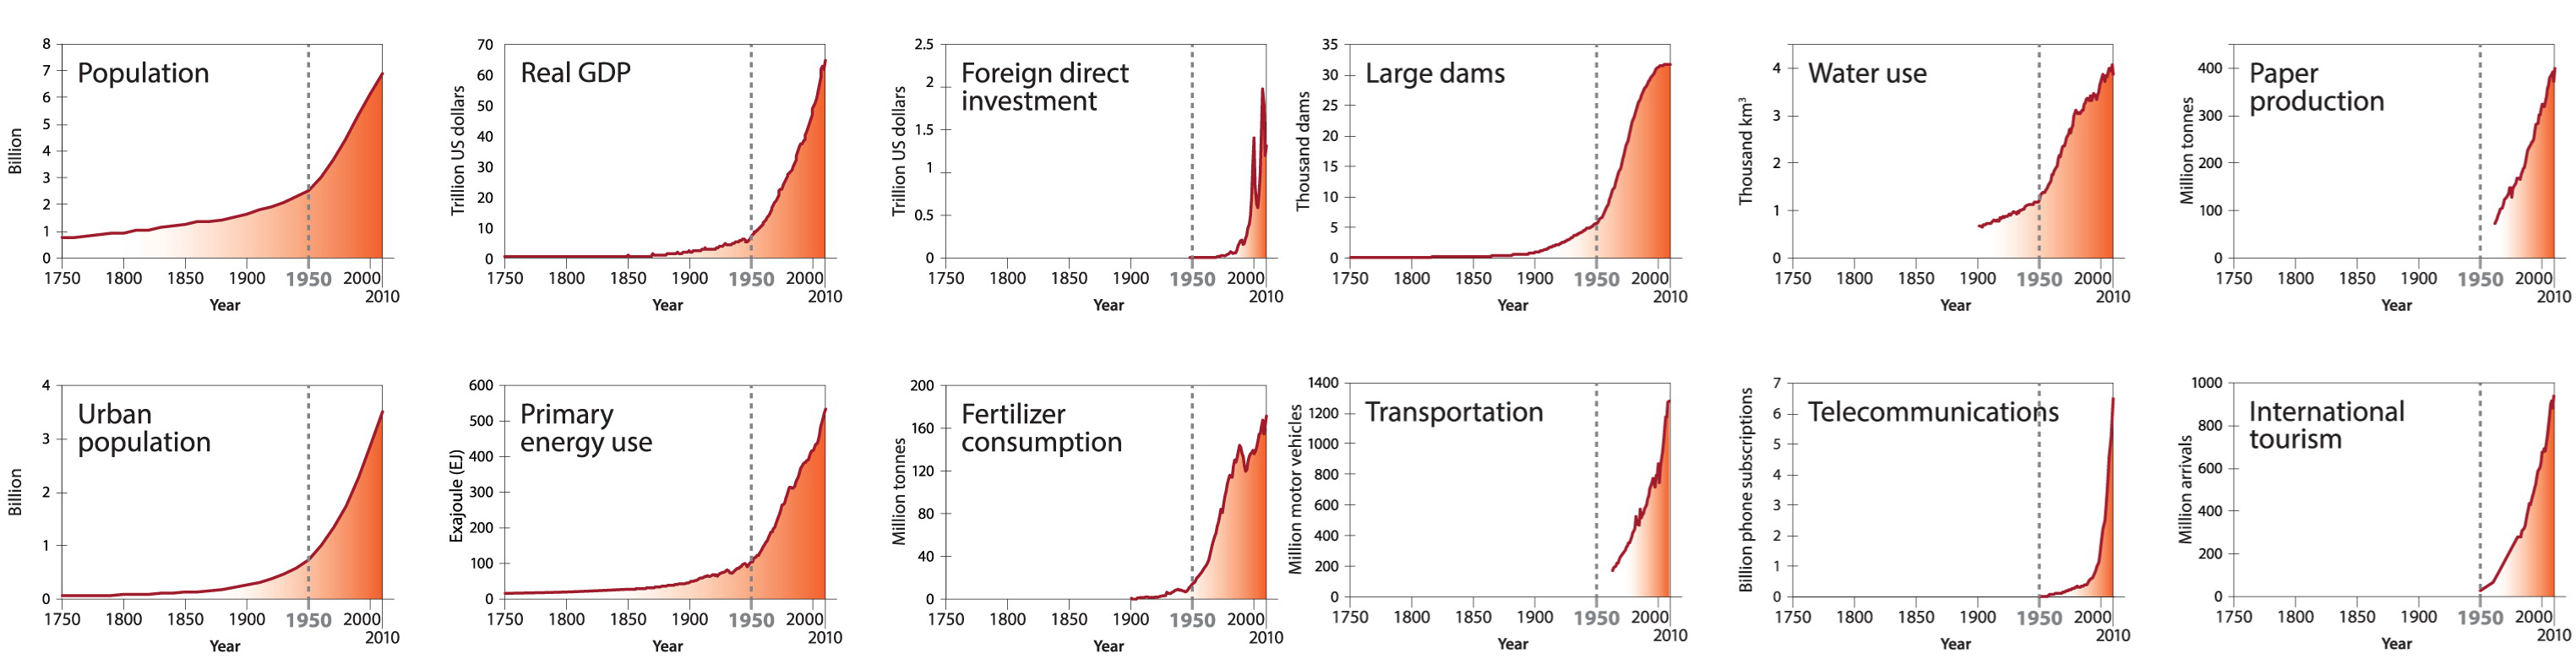
\includegraphics[width=\linewidth]{figures/Anthropocene1V.jpg}
    \caption{Évolution, de 1750 à 2010, de différents indicateurs mondiaux
    du développement socio-économique\cite{steffen_trajectory_2015}.}
    \label{fig:anthropocene1}
\end{figure}
 
\begin{figure}[htbp]
    \centering
    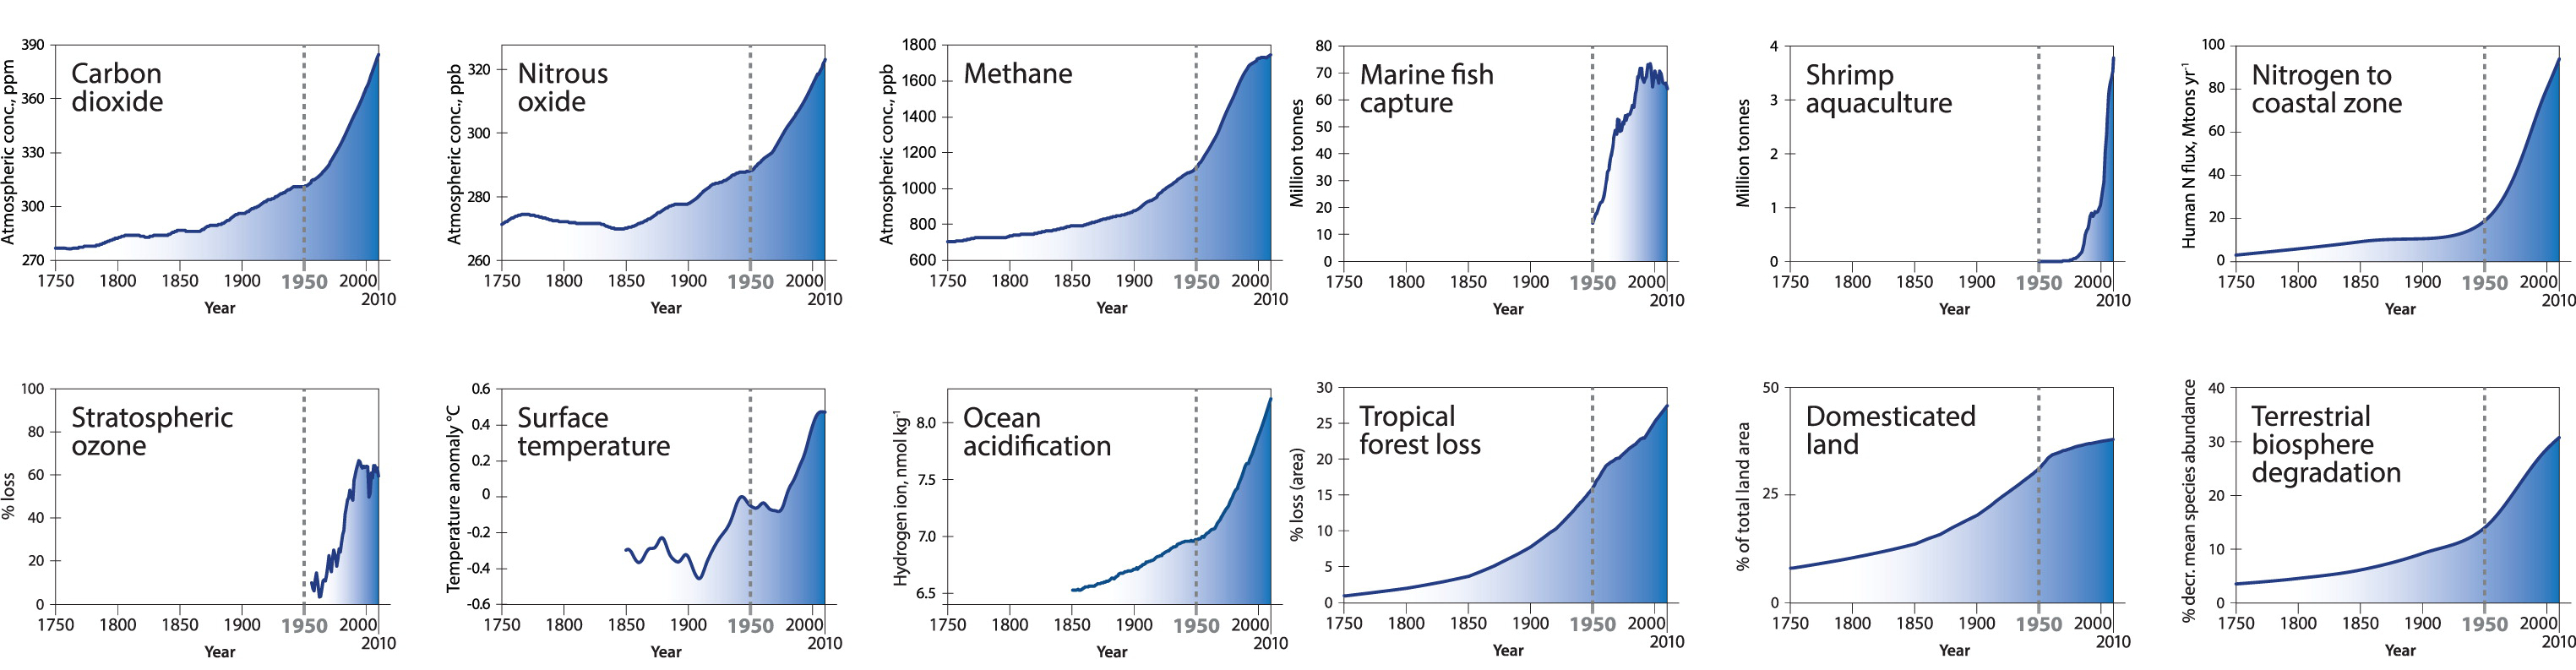
\includegraphics[width=\linewidth]{figures/Anthropocene2V.jpg}
    \caption{Évolution, de 1750 à 2010, de différents indicateurs du
    système terrestre\cite{steffen_trajectory_2015}.}
    \label{fig:anthropocene2}
\end{figure}
 
Ces deux séries présentent la même allure : une évolution lente jusqu'au milieu du \textsc{xx}\textsuperscript{e}~siècle, puis une envolée brutale à partir des années 1950. Cette simultanéité, que les auteurs nomment la \emph{Grande Accélération}, met en évidence le lien direct entre la croissance des activités humaines et la dégradation du système terrestre.

\chapter{Dérèglement climatique}
\section{L'effet de serre}
\label{chap:effet-serre}
\subsection*{La loi de Stefan - Boltzmann}
Pour rappel, les corps rayonnent en fonction de leur température\footfullcite{stefan1879}:
\begin{equation}
  P = \sigma T^4
\end{equation}
avec $P$ la puissance surfacique (W/m$^2$), $\sigma$ la constante de Stefan - Boltzmann (W/m$^2$.K$^4$) et $T$ la température (K).

\subsection*{Mécanisme de l'effet de serre}
Le mécanisme de l'effet de serre peut se décomposer en plusieurs étapes \footfullcite{oce}, \footfullcite{reveilleur-effet-serre}, \footfullcite{ipcc_climate_2021} et est illustré dans la figure \ref{fig:serre}.
\begin{enumerate}
  \item \textbf{Rayonnement venant du Soleil} : le rayonnement solaire atteint le haut de l'atmosphère.
  \item \textbf{Traversée de l'atmosphère terrestre} : une partie du rayonnement est réfléchie vers l'espace, une autre est transmise vers la surface de la Terre.
  \item \textbf{Arrivée à la surface de la Terre} : une partie du rayonnement est réfléchie vers l'atmosphère, l'autre est absorbée par la surface.
  \item \textbf{Accumulation d'énergie} : la température de la surface terrestre augmente car elle reçoit l'énergie du Soleil.
  \item \textbf{Émission de rayonnement infrarouge} : la surface émet alors un rayonnement infrarouge, qui transporte de la chaleur vers l'atmosphère, ce qui refroidit la surface de la Terre.
  \item \textbf{Effet de serre} : certains gaz de l'atmosphère absorbent une partie du rayonnement infrarouge, empêchant que toute la chaleur de ce rayonnement ne s'échappe dans l'espace.
  \item \textbf{Nouvelle absorption par la surface} : la surface de la Terre se réchauffe alors davantage.
\end{enumerate}

\begin{figure}[h]
    \centering
    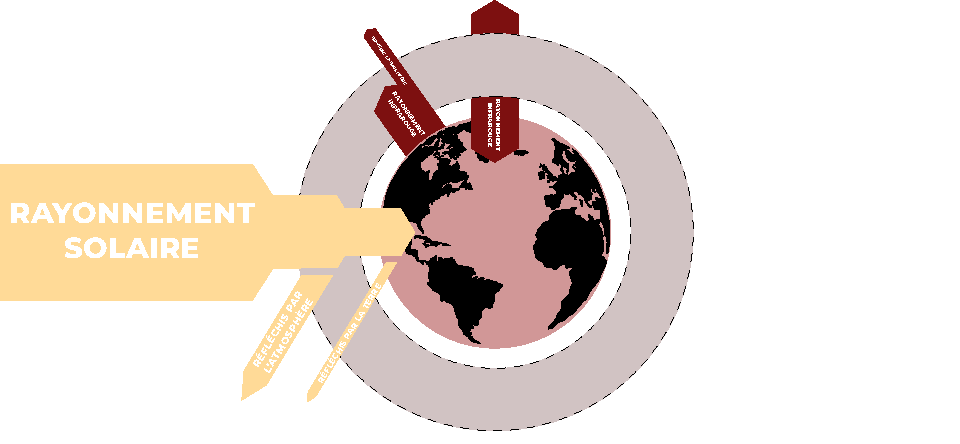
\includegraphics[width=1\linewidth]{figures/serre.pdf}
    \caption{Schéma de principe de l'effet de serre}
    \label{fig:serre}
\end{figure}

La Terre, plus froide que le Soleil, rayonne dans l'infrarouge. Sans effet de serre, la température de la Terre serait à l'équilibre autour de $-18$\,°C. Avec l'effet de serre, la température de la Terre s'équilibre autour de 15\,°C.

Ainsi, l'effet de serre n'est ni « bon » ni « mauvais » : c'est un mécanisme naturel qui maintient la température moyenne de la surface de la Terre autour de 15\,°C, au lieu d'environ $-18$\,°C. 
Le principal gaz à effet de serre est la vapeur d'eau. Sa quantité dans l'atmosphère est globalement stable depuis des milliers d'années. La partie suivante montre l'impact de l'être humain sur l'augmentation de la quantité de gaz à effet de serre dans l'atmosphère. C'est cette augmentation de gaz à effet de serre qui augmente le forçage radiatif conduisant la Terre à se réchauffer.

Les gaz à effet de serre sont simplement définis comme les gaz absorbant le rayonnement infrarouge, c'est une propriété intrinsèque à chaque gaz (certains absorbent le rayonnement infrarouge, d'autres non).

\subsection*{Limite de l'analogie}

\section{Évolution et contribution antropique}

\chapter{Atténuation et Adaptation face au changement climatique}
\section{Atténuation}
\section{Adaptation}
% TODO : à compléter
